\documentclass[11pt]{article}
\usepackage[textwidth=18.0cm, textheight=23.0cm, top=2.0cm]{geometry}
\usepackage{pst-all}
\usepackage{amssymb}
\usepackage{tikz}
\usepackage{underscore}\begin{document}
\pagestyle{empty}


ClassName: \underline{\textbf{Class_08.2bp-22}}
\par
BinSize: \underline{\textbf{100 × 100}}
\par
ReduceSize: \underline{\textbf{100 × 100}}
\par
TypeNum: \underline{\textbf{60}}
\par
Num: \underline{\textbf{60}}
\par
OutS: \underline{\textbf{170000}}
\par
InS: \underline{\textbf{140453}}
\par
Rate: \underline{\textbf{0.826}}
\par
UB: \underline{\textbf{17}}
\par
LB0: \underline{\textbf{16}}
\par
LB: \underline{\textbf{16}}
\par
LBWithCut: \underline{\textbf{17}}
\par
NodeCut: \underline{\textbf{1}}
\par
ExtendedNodeCnt: \underline{\textbf{1}}
\par
GenNodeCnt: \underline{\textbf{1}}
\par
PrimalNode: \underline{\textbf{0}}
\par
ColumnCount: \underline{\textbf{196}}
\par
TotalCutCount: \underline{\textbf{48}}
\par
RootCutCount: \underline{\textbf{48}}
\par
LPSolverCnt: \underline{\textbf{181}}
\par
PricingSolverCnt: \underline{\textbf{181}}
\par
BranchAndBoundNum: \underline{\textbf{1}}
\par
isOpt: \underline{\textbf{true}}
\par
TimeOnInitSolution: \underline{\textbf{120.010 s}}
\par
TimeOnPrimal: \underline{\textbf{0.000 s}}
\par
TimeOnPricing: \underline{\textbf{15.431 s}}
\par
TimeOnRmp: \underline{\textbf{0.182 s}}
\par
TotalTime: \underline{\textbf{135.806 s}}
\par
\newpage


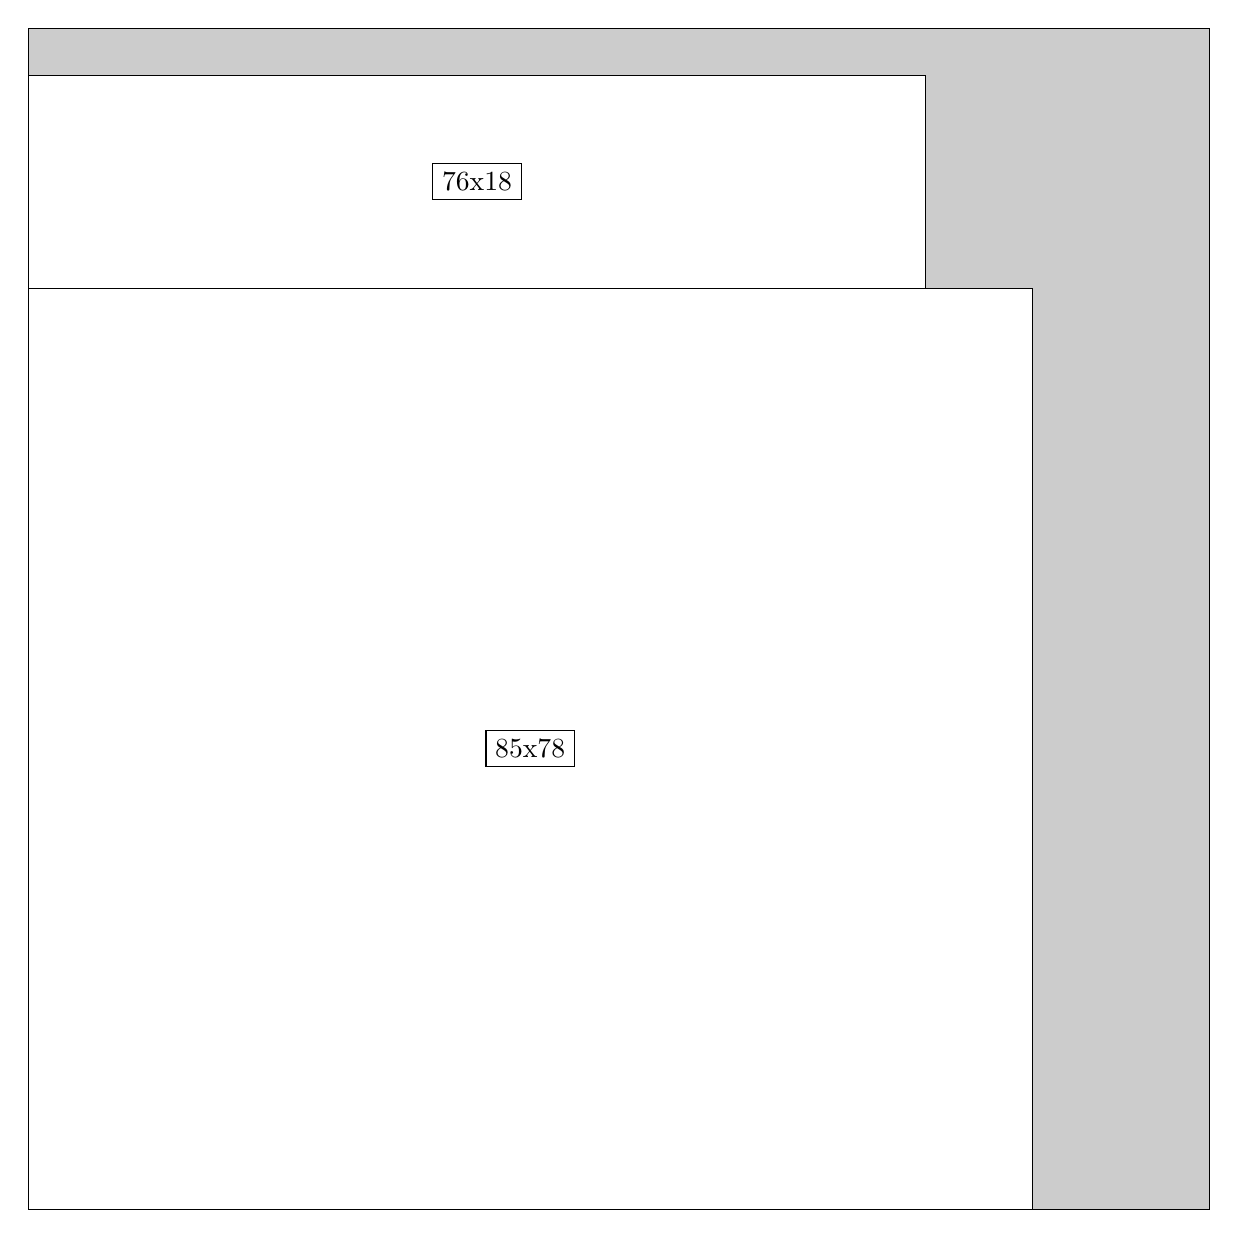
\begin{tikzpicture}[shorten >=1pt,scale=1.0,every node/.style={scale=1.0},->]
\tikzstyle{vertex}=[circle,fill=black!25,minimum size=14pt,inner sep=0pt]
\filldraw[fill=gray!40!white, draw=black] (0,0) rectangle (15.0,15.0);
\foreach \name/\x/\y/\w/\h in {85x78/0.0/0.0/12.75/11.7,76x18/0.0/11.7/11.4/2.6999999999999997}
\filldraw[fill=white!40!white, draw=black] (\x,\y) rectangle node[draw] (\name) {\name} ++(\w,\h);
\end{tikzpicture}


w =85 , h =78 , x =0 , y =0 , v =6630
\par
w =76 , h =18 , x =0 , y =78 , v =1368
\par
\newpage


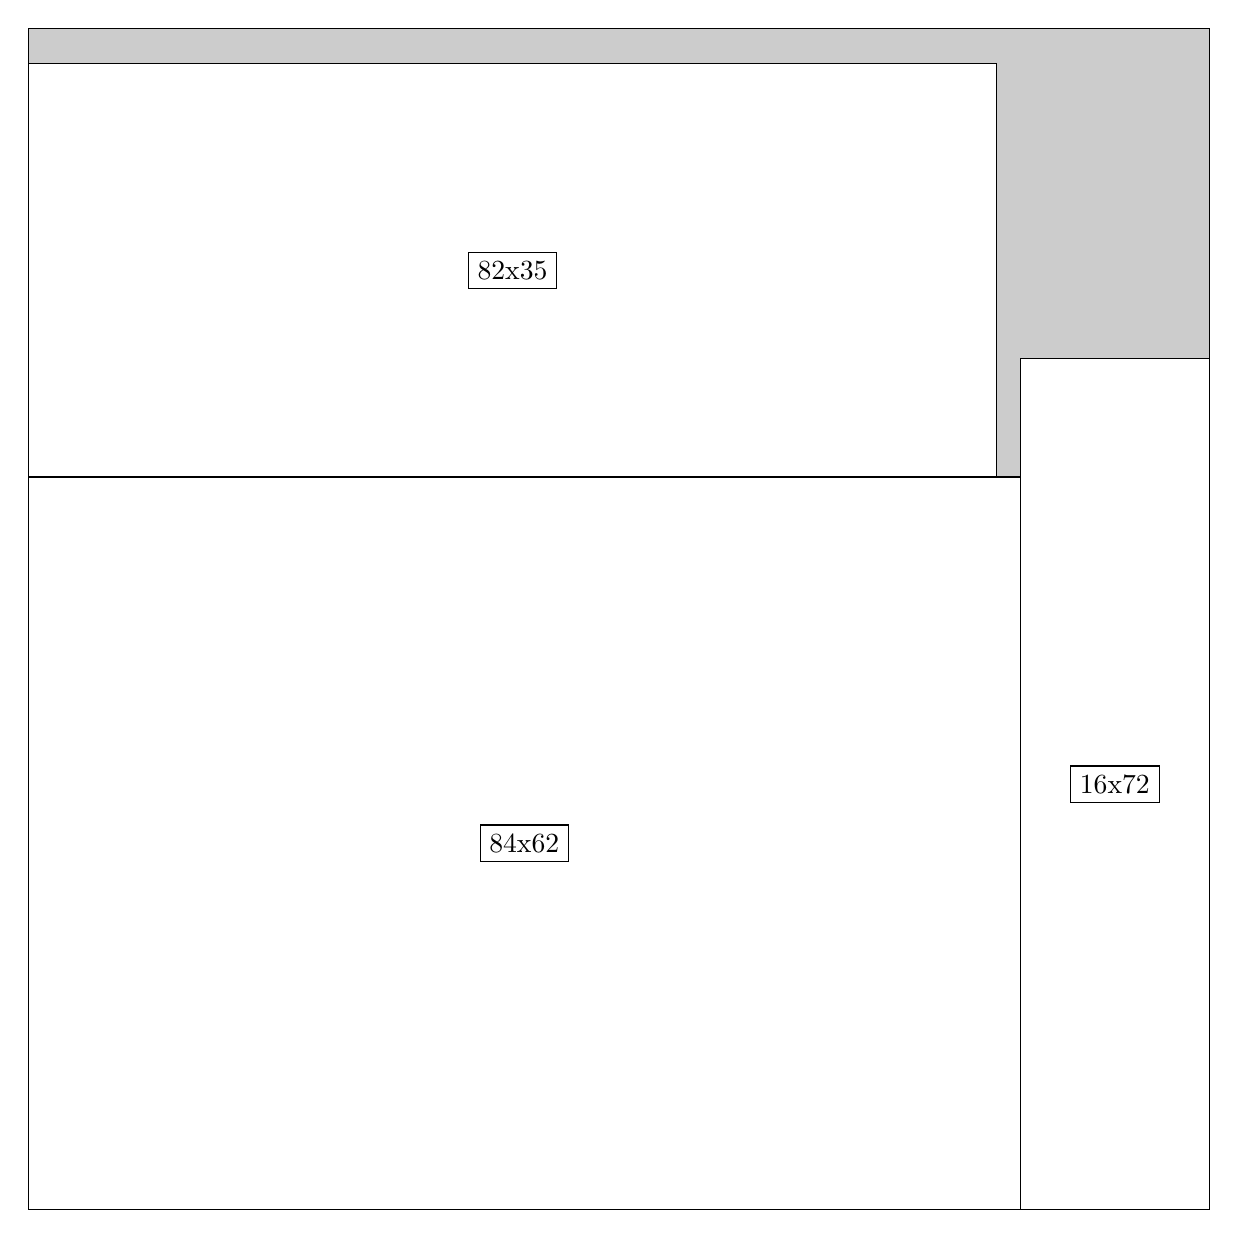
\begin{tikzpicture}[shorten >=1pt,scale=1.0,every node/.style={scale=1.0},->]
\tikzstyle{vertex}=[circle,fill=black!25,minimum size=14pt,inner sep=0pt]
\filldraw[fill=gray!40!white, draw=black] (0,0) rectangle (15.0,15.0);
\foreach \name/\x/\y/\w/\h in {84x62/0.0/0.0/12.6/9.299999999999999,82x35/0.0/9.299999999999999/12.299999999999999/5.25,16x72/12.6/0.0/2.4/10.799999999999999}
\filldraw[fill=white!40!white, draw=black] (\x,\y) rectangle node[draw] (\name) {\name} ++(\w,\h);
\end{tikzpicture}


w =84 , h =62 , x =0 , y =0 , v =5208
\par
w =82 , h =35 , x =0 , y =62 , v =2870
\par
w =16 , h =72 , x =84 , y =0 , v =1152
\par
\newpage


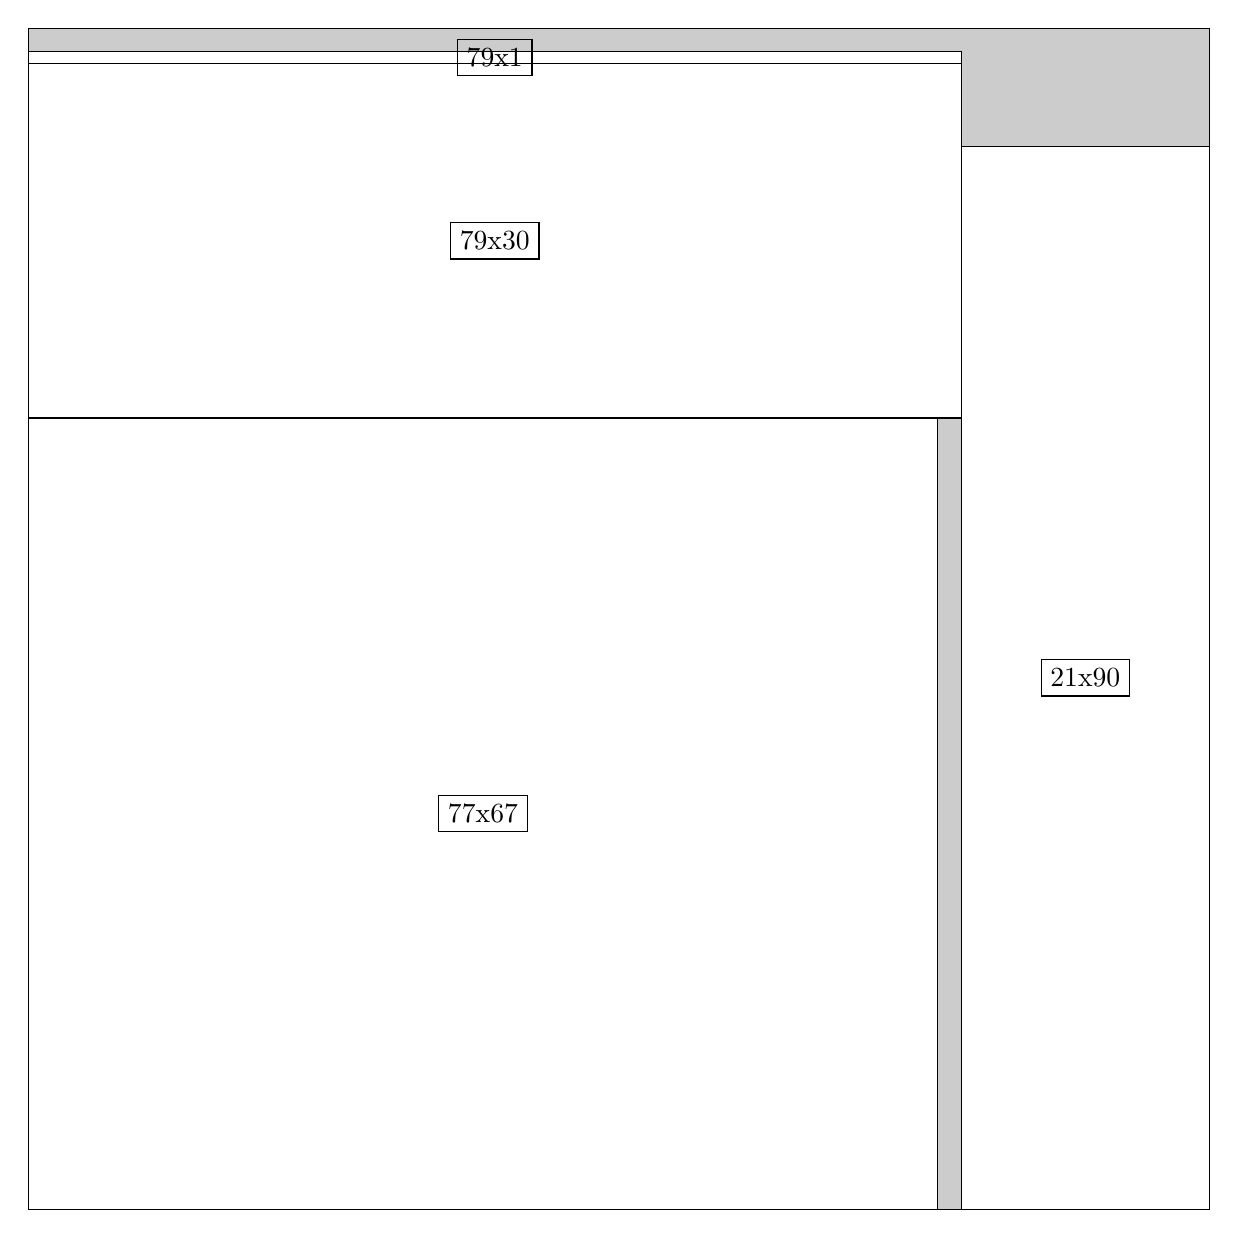
\begin{tikzpicture}[shorten >=1pt,scale=1.0,every node/.style={scale=1.0},->]
\tikzstyle{vertex}=[circle,fill=black!25,minimum size=14pt,inner sep=0pt]
\filldraw[fill=gray!40!white, draw=black] (0,0) rectangle (15.0,15.0);
\foreach \name/\x/\y/\w/\h in {77x67/0.0/0.0/11.549999999999999/10.049999999999999,79x30/0.0/10.049999999999999/11.85/4.5,21x90/11.85/0.0/3.15/13.5,79x1/0.0/14.549999999999999/11.85/0.15}
\filldraw[fill=white!40!white, draw=black] (\x,\y) rectangle node[draw] (\name) {\name} ++(\w,\h);
\end{tikzpicture}


w =77 , h =67 , x =0 , y =0 , v =5159
\par
w =79 , h =30 , x =0 , y =67 , v =2370
\par
w =21 , h =90 , x =79 , y =0 , v =1890
\par
w =79 , h =1 , x =0 , y =97 , v =79
\par
\newpage


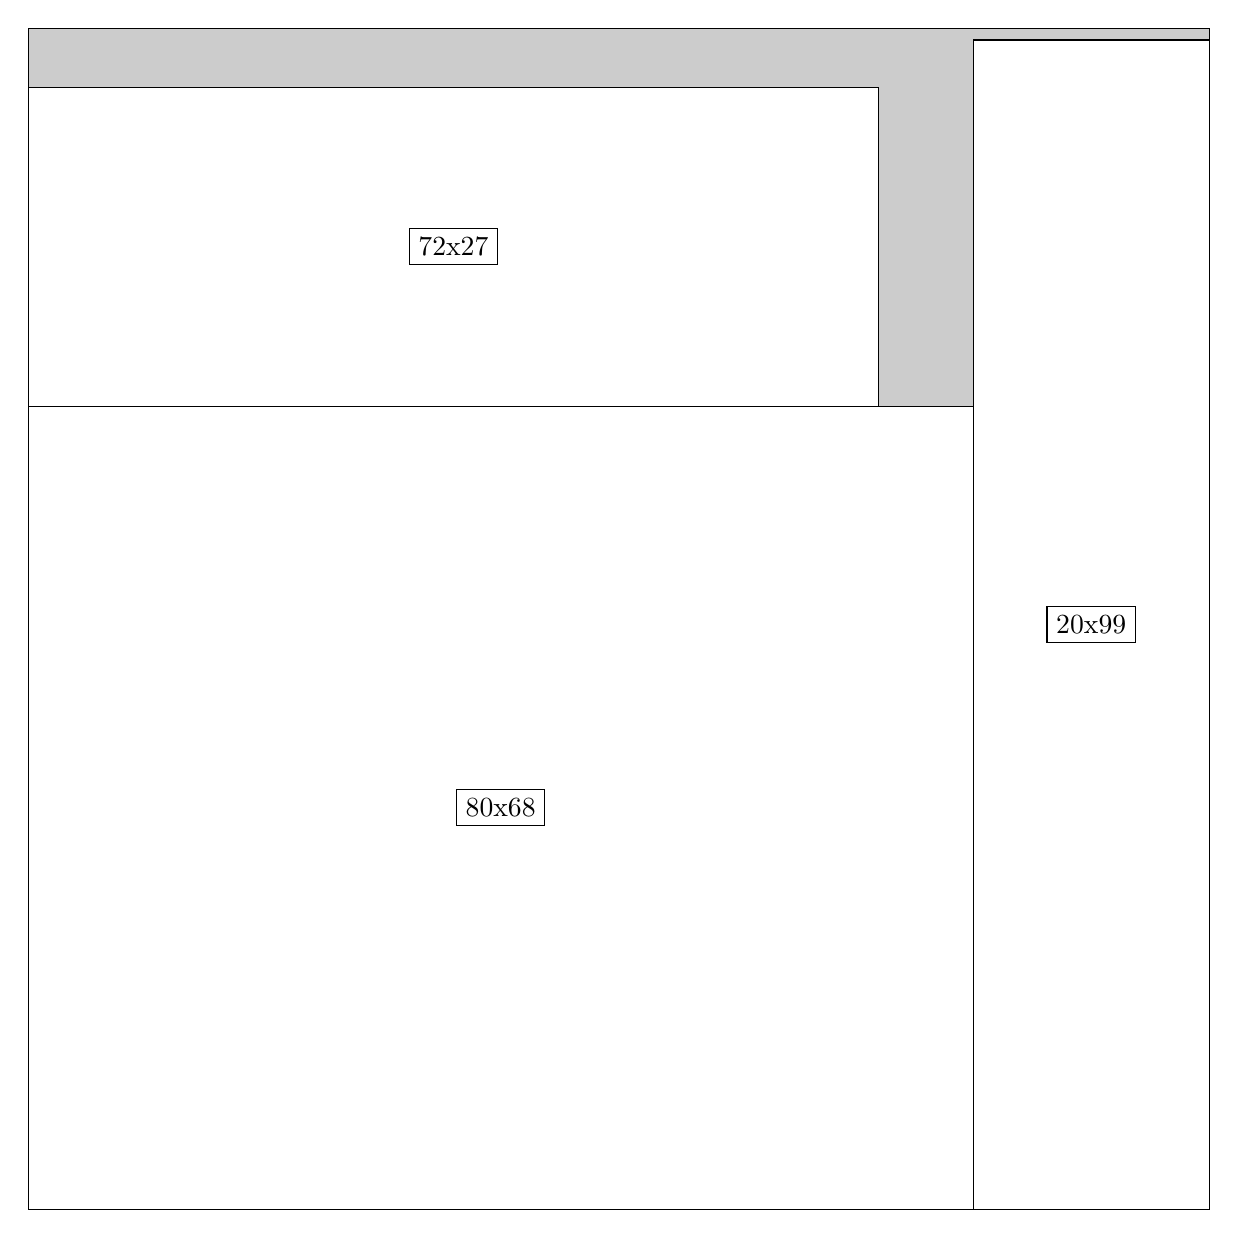
\begin{tikzpicture}[shorten >=1pt,scale=1.0,every node/.style={scale=1.0},->]
\tikzstyle{vertex}=[circle,fill=black!25,minimum size=14pt,inner sep=0pt]
\filldraw[fill=gray!40!white, draw=black] (0,0) rectangle (15.0,15.0);
\foreach \name/\x/\y/\w/\h in {80x68/0.0/0.0/12.0/10.2,20x99/12.0/0.0/3.0/14.85,72x27/0.0/10.2/10.799999999999999/4.05}
\filldraw[fill=white!40!white, draw=black] (\x,\y) rectangle node[draw] (\name) {\name} ++(\w,\h);
\end{tikzpicture}


w =80 , h =68 , x =0 , y =0 , v =5440
\par
w =20 , h =99 , x =80 , y =0 , v =1980
\par
w =72 , h =27 , x =0 , y =68 , v =1944
\par
\newpage


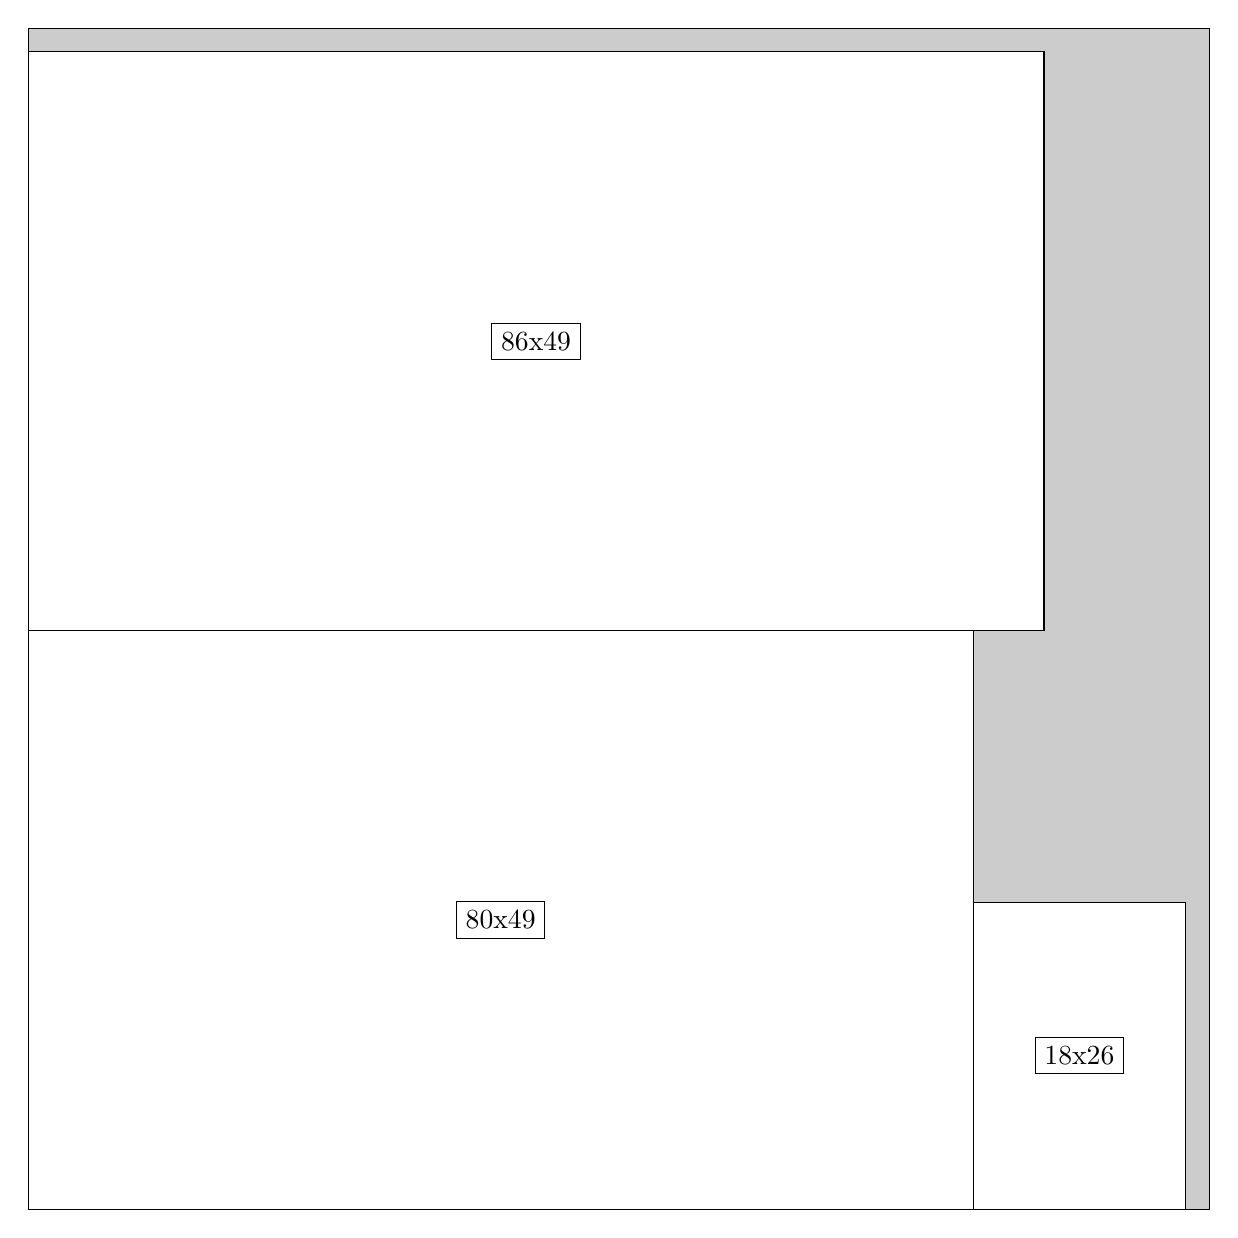
\begin{tikzpicture}[shorten >=1pt,scale=1.0,every node/.style={scale=1.0},->]
\tikzstyle{vertex}=[circle,fill=black!25,minimum size=14pt,inner sep=0pt]
\filldraw[fill=gray!40!white, draw=black] (0,0) rectangle (15.0,15.0);
\foreach \name/\x/\y/\w/\h in {86x49/0.0/7.35/12.9/7.35,80x49/0.0/0.0/12.0/7.35,18x26/12.0/0.0/2.6999999999999997/3.9}
\filldraw[fill=white!40!white, draw=black] (\x,\y) rectangle node[draw] (\name) {\name} ++(\w,\h);
\end{tikzpicture}


w =86 , h =49 , x =0 , y =49 , v =4214
\par
w =80 , h =49 , x =0 , y =0 , v =3920
\par
w =18 , h =26 , x =80 , y =0 , v =468
\par
\newpage


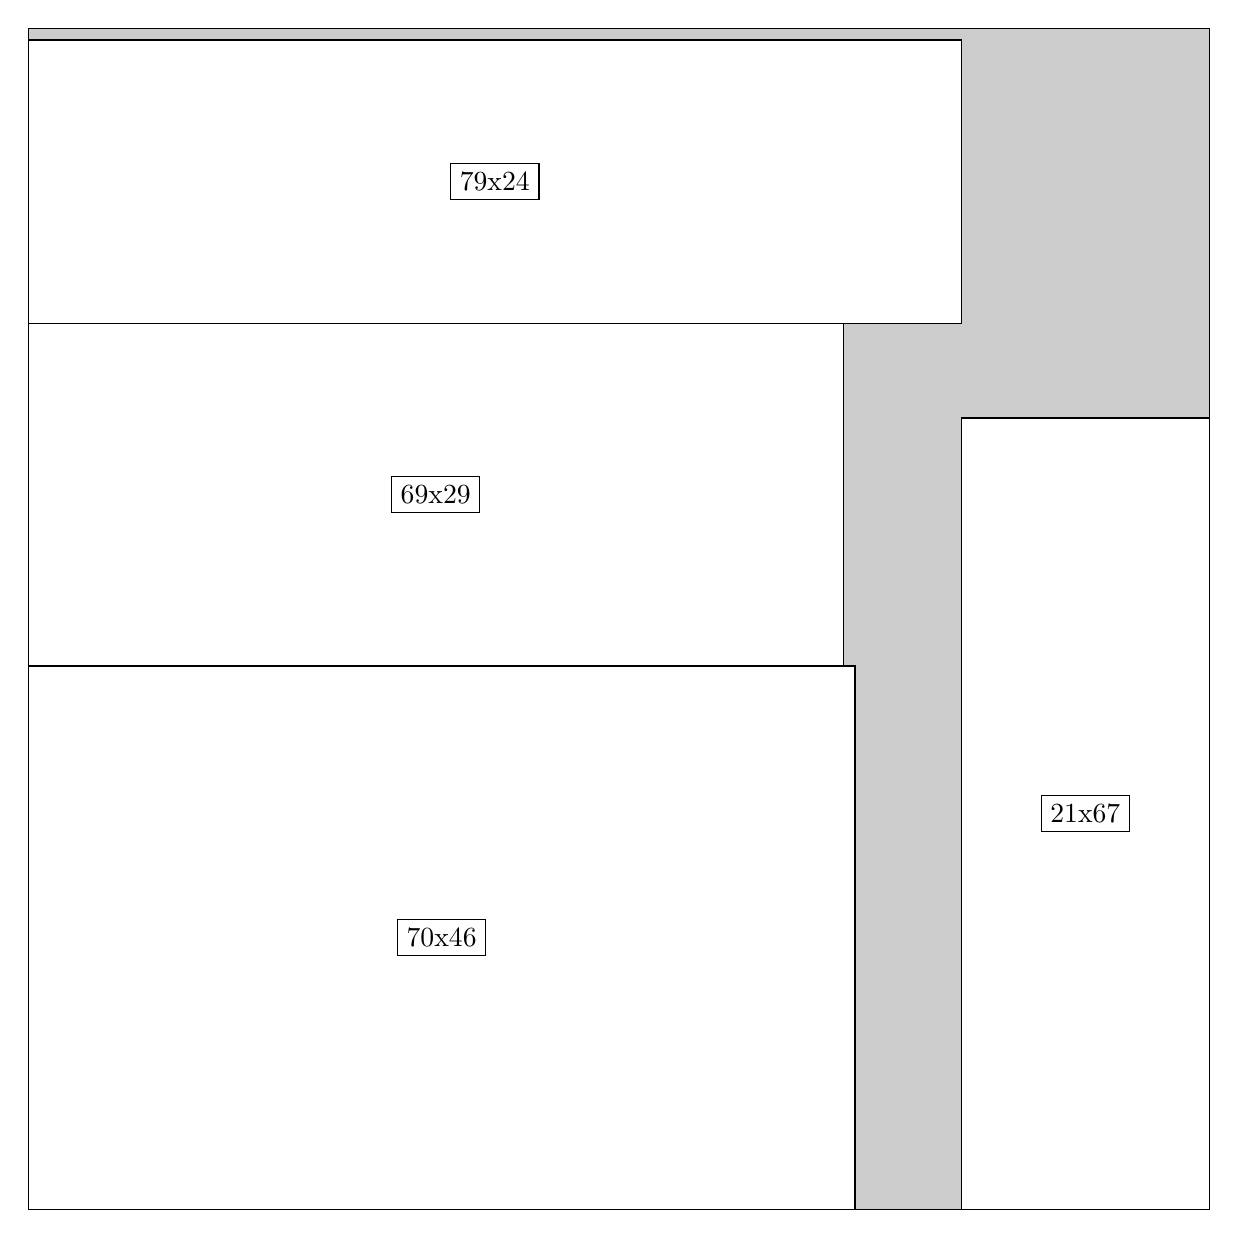
\begin{tikzpicture}[shorten >=1pt,scale=1.0,every node/.style={scale=1.0},->]
\tikzstyle{vertex}=[circle,fill=black!25,minimum size=14pt,inner sep=0pt]
\filldraw[fill=gray!40!white, draw=black] (0,0) rectangle (15.0,15.0);
\foreach \name/\x/\y/\w/\h in {70x46/0.0/0.0/10.5/6.8999999999999995,69x29/0.0/6.8999999999999995/10.35/4.35,79x24/0.0/11.25/11.85/3.5999999999999996,21x67/11.85/0.0/3.15/10.049999999999999}
\filldraw[fill=white!40!white, draw=black] (\x,\y) rectangle node[draw] (\name) {\name} ++(\w,\h);
\end{tikzpicture}


w =70 , h =46 , x =0 , y =0 , v =3220
\par
w =69 , h =29 , x =0 , y =46 , v =2001
\par
w =79 , h =24 , x =0 , y =75 , v =1896
\par
w =21 , h =67 , x =79 , y =0 , v =1407
\par
\newpage


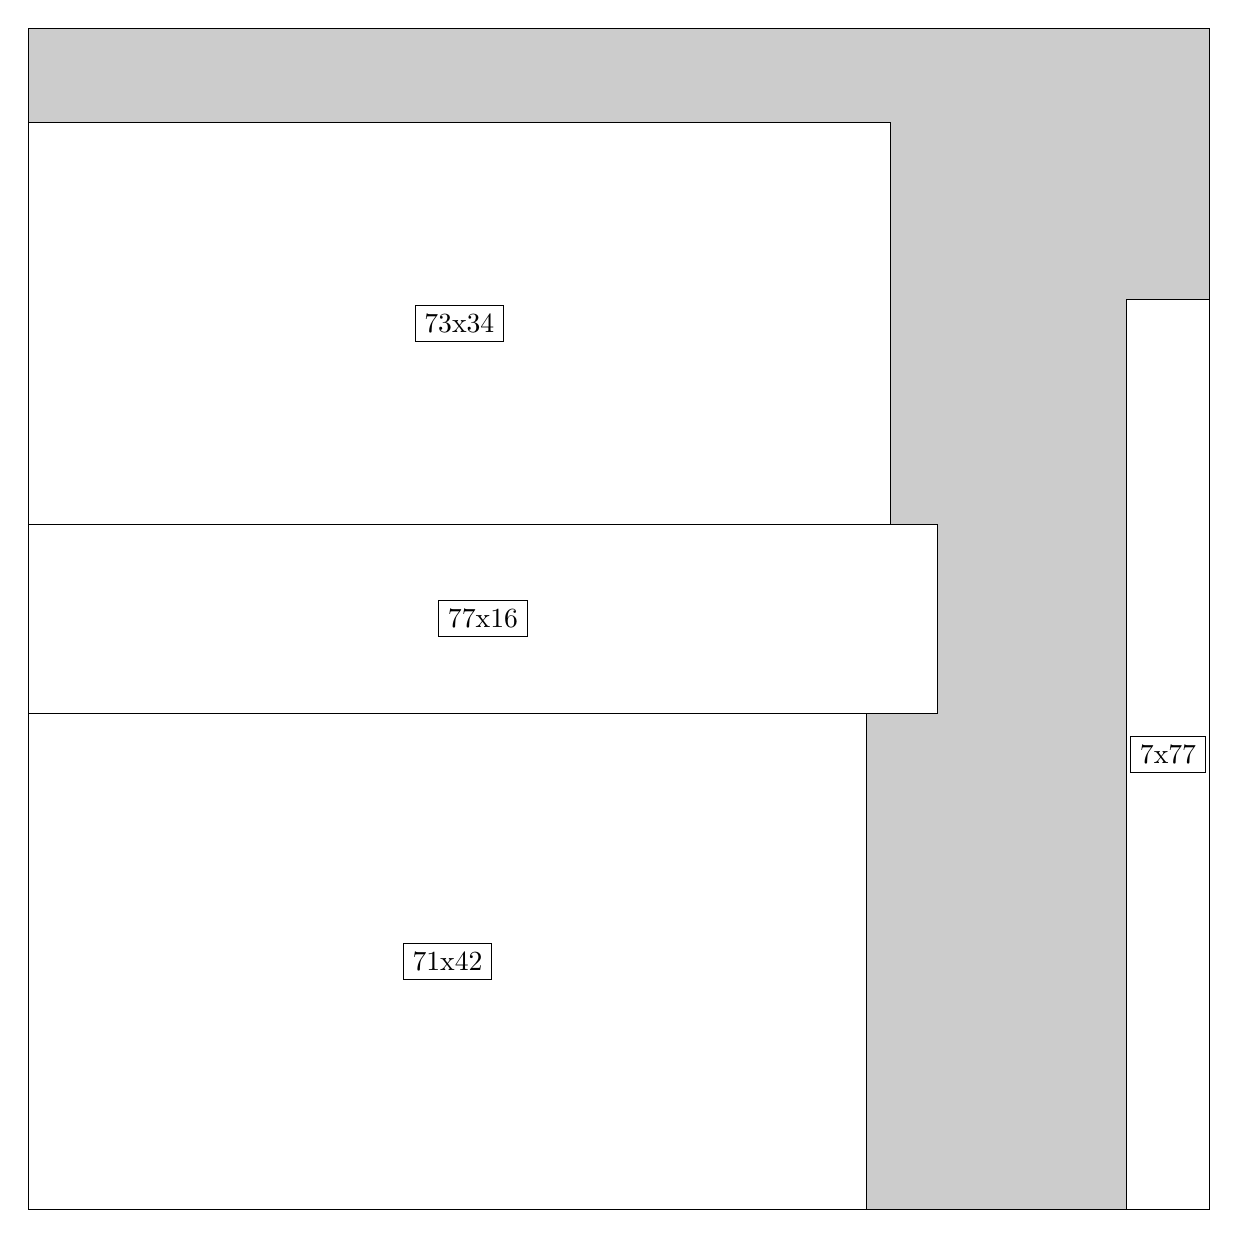
\begin{tikzpicture}[shorten >=1pt,scale=1.0,every node/.style={scale=1.0},->]
\tikzstyle{vertex}=[circle,fill=black!25,minimum size=14pt,inner sep=0pt]
\filldraw[fill=gray!40!white, draw=black] (0,0) rectangle (15.0,15.0);
\foreach \name/\x/\y/\w/\h in {71x42/0.0/0.0/10.65/6.3,73x34/0.0/8.7/10.95/5.1,77x16/0.0/6.3/11.549999999999999/2.4,7x77/13.95/0.0/1.05/11.549999999999999}
\filldraw[fill=white!40!white, draw=black] (\x,\y) rectangle node[draw] (\name) {\name} ++(\w,\h);
\end{tikzpicture}


w =71 , h =42 , x =0 , y =0 , v =2982
\par
w =73 , h =34 , x =0 , y =58 , v =2482
\par
w =77 , h =16 , x =0 , y =42 , v =1232
\par
w =7 , h =77 , x =93 , y =0 , v =539
\par
\newpage


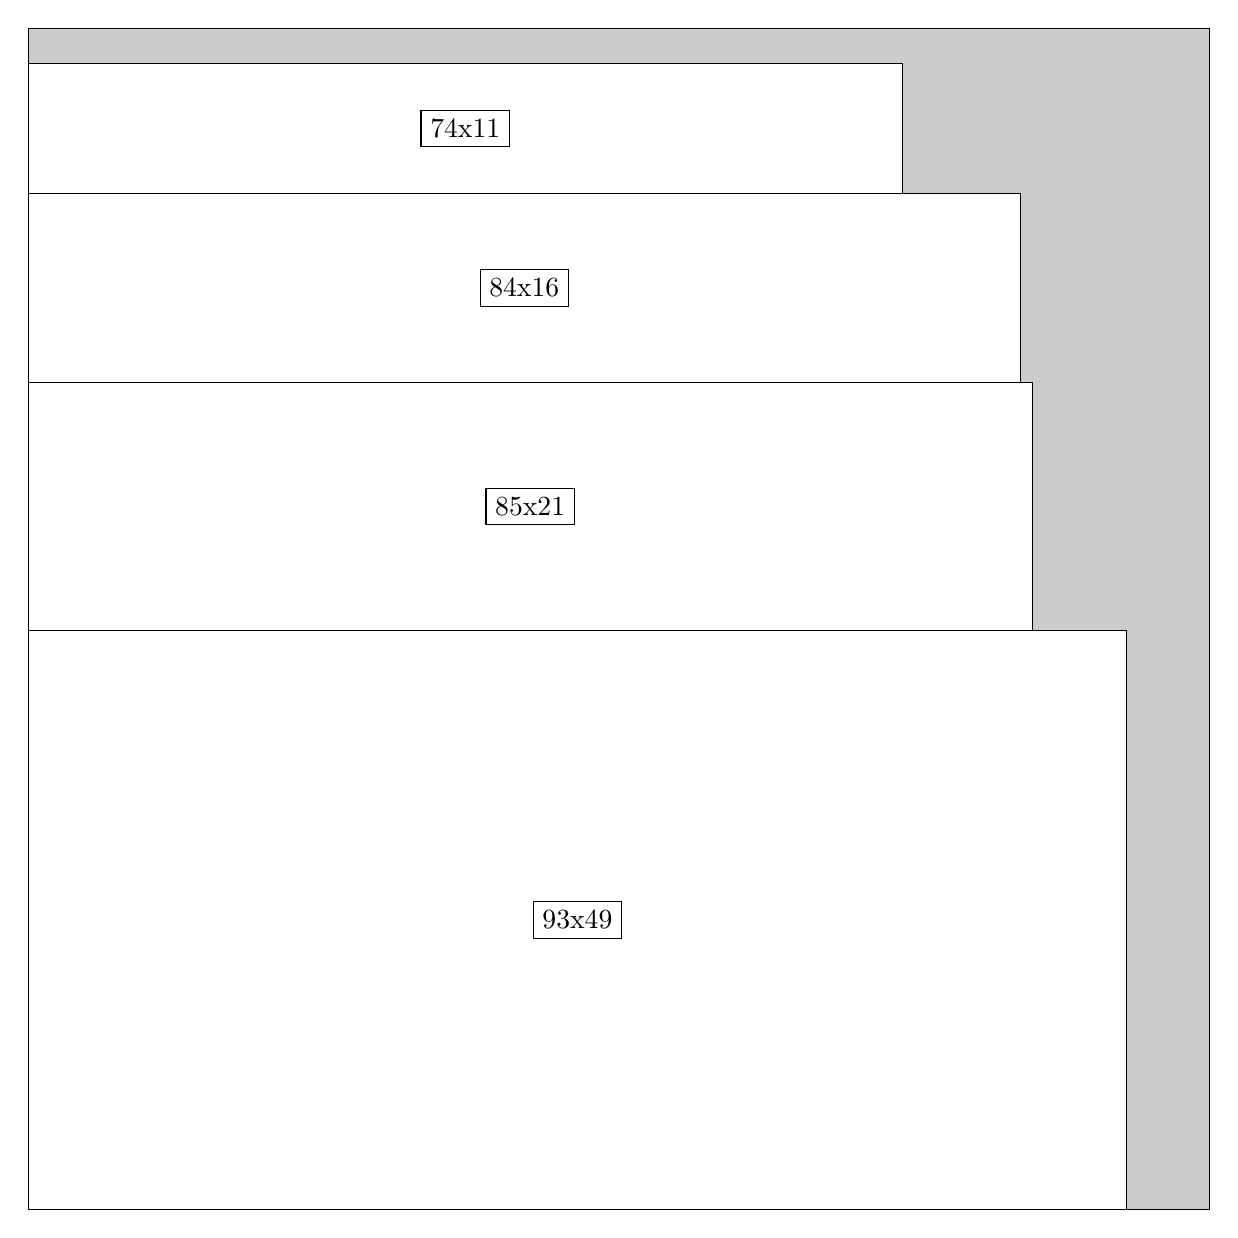
\begin{tikzpicture}[shorten >=1pt,scale=1.0,every node/.style={scale=1.0},->]
\tikzstyle{vertex}=[circle,fill=black!25,minimum size=14pt,inner sep=0pt]
\filldraw[fill=gray!40!white, draw=black] (0,0) rectangle (15.0,15.0);
\foreach \name/\x/\y/\w/\h in {93x49/0.0/0.0/13.95/7.35,85x21/0.0/7.35/12.75/3.15,84x16/0.0/10.5/12.6/2.4,74x11/0.0/12.9/11.1/1.65}
\filldraw[fill=white!40!white, draw=black] (\x,\y) rectangle node[draw] (\name) {\name} ++(\w,\h);
\end{tikzpicture}


w =93 , h =49 , x =0 , y =0 , v =4557
\par
w =85 , h =21 , x =0 , y =49 , v =1785
\par
w =84 , h =16 , x =0 , y =70 , v =1344
\par
w =74 , h =11 , x =0 , y =86 , v =814
\par
\newpage


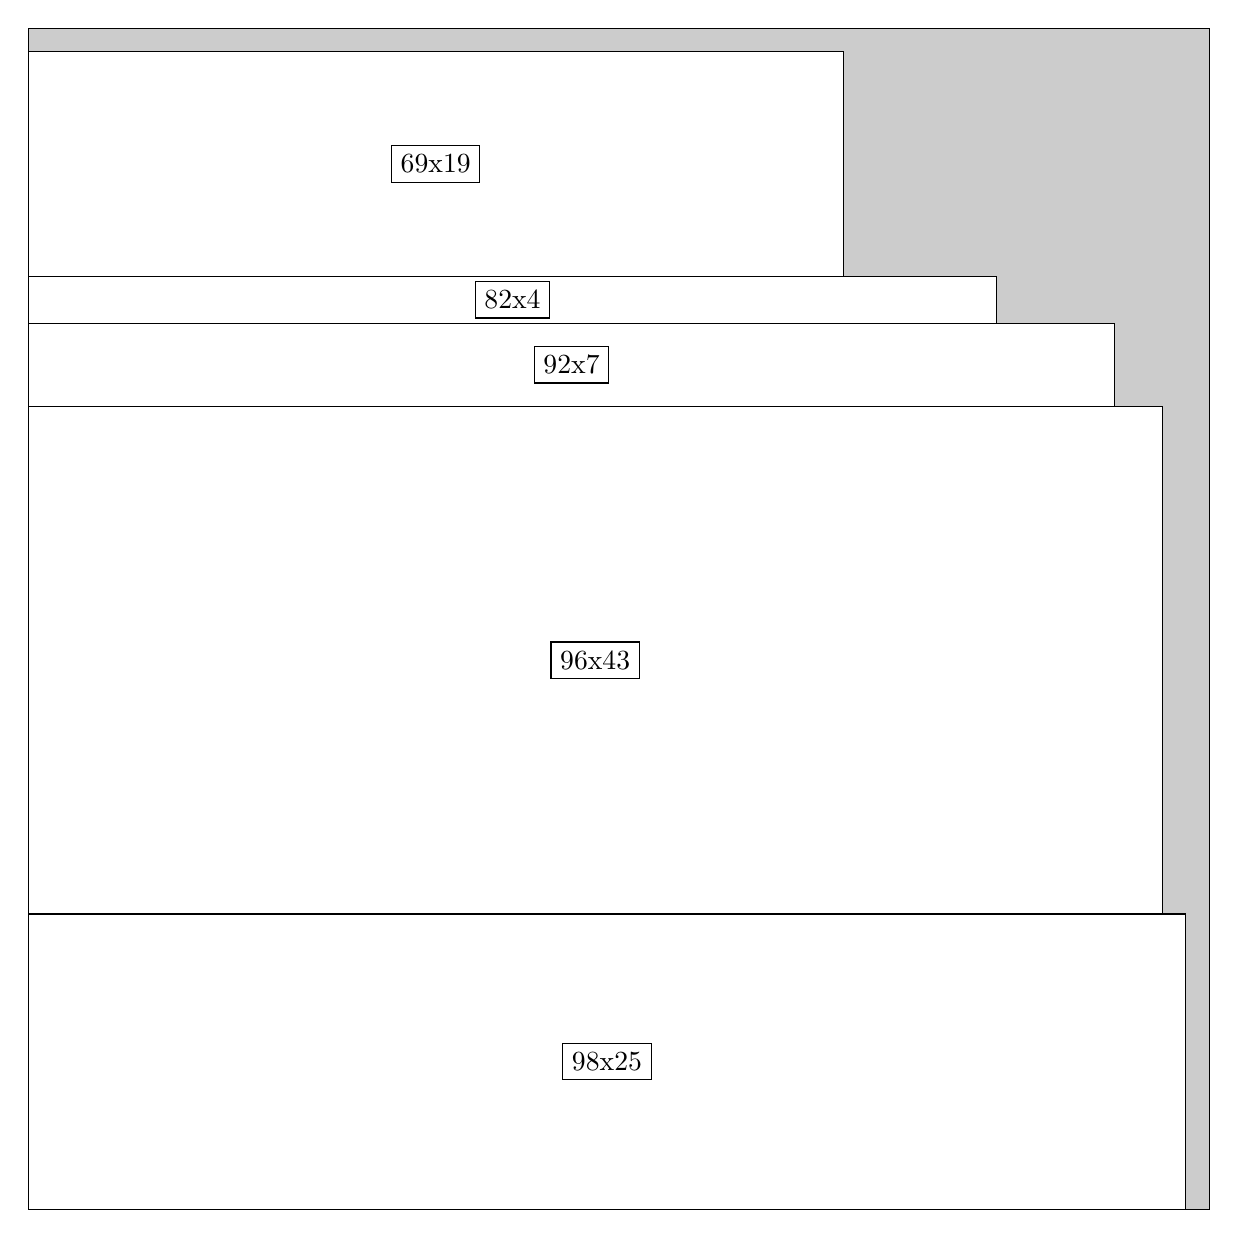
\begin{tikzpicture}[shorten >=1pt,scale=1.0,every node/.style={scale=1.0},->]
\tikzstyle{vertex}=[circle,fill=black!25,minimum size=14pt,inner sep=0pt]
\filldraw[fill=gray!40!white, draw=black] (0,0) rectangle (15.0,15.0);
\foreach \name/\x/\y/\w/\h in {96x43/0.0/3.75/14.399999999999999/6.45,98x25/0.0/0.0/14.7/3.75,69x19/0.0/11.85/10.35/2.85,92x7/0.0/10.2/13.799999999999999/1.05,82x4/0.0/11.25/12.299999999999999/0.6}
\filldraw[fill=white!40!white, draw=black] (\x,\y) rectangle node[draw] (\name) {\name} ++(\w,\h);
\end{tikzpicture}


w =96 , h =43 , x =0 , y =25 , v =4128
\par
w =98 , h =25 , x =0 , y =0 , v =2450
\par
w =69 , h =19 , x =0 , y =79 , v =1311
\par
w =92 , h =7 , x =0 , y =68 , v =644
\par
w =82 , h =4 , x =0 , y =75 , v =328
\par
\newpage


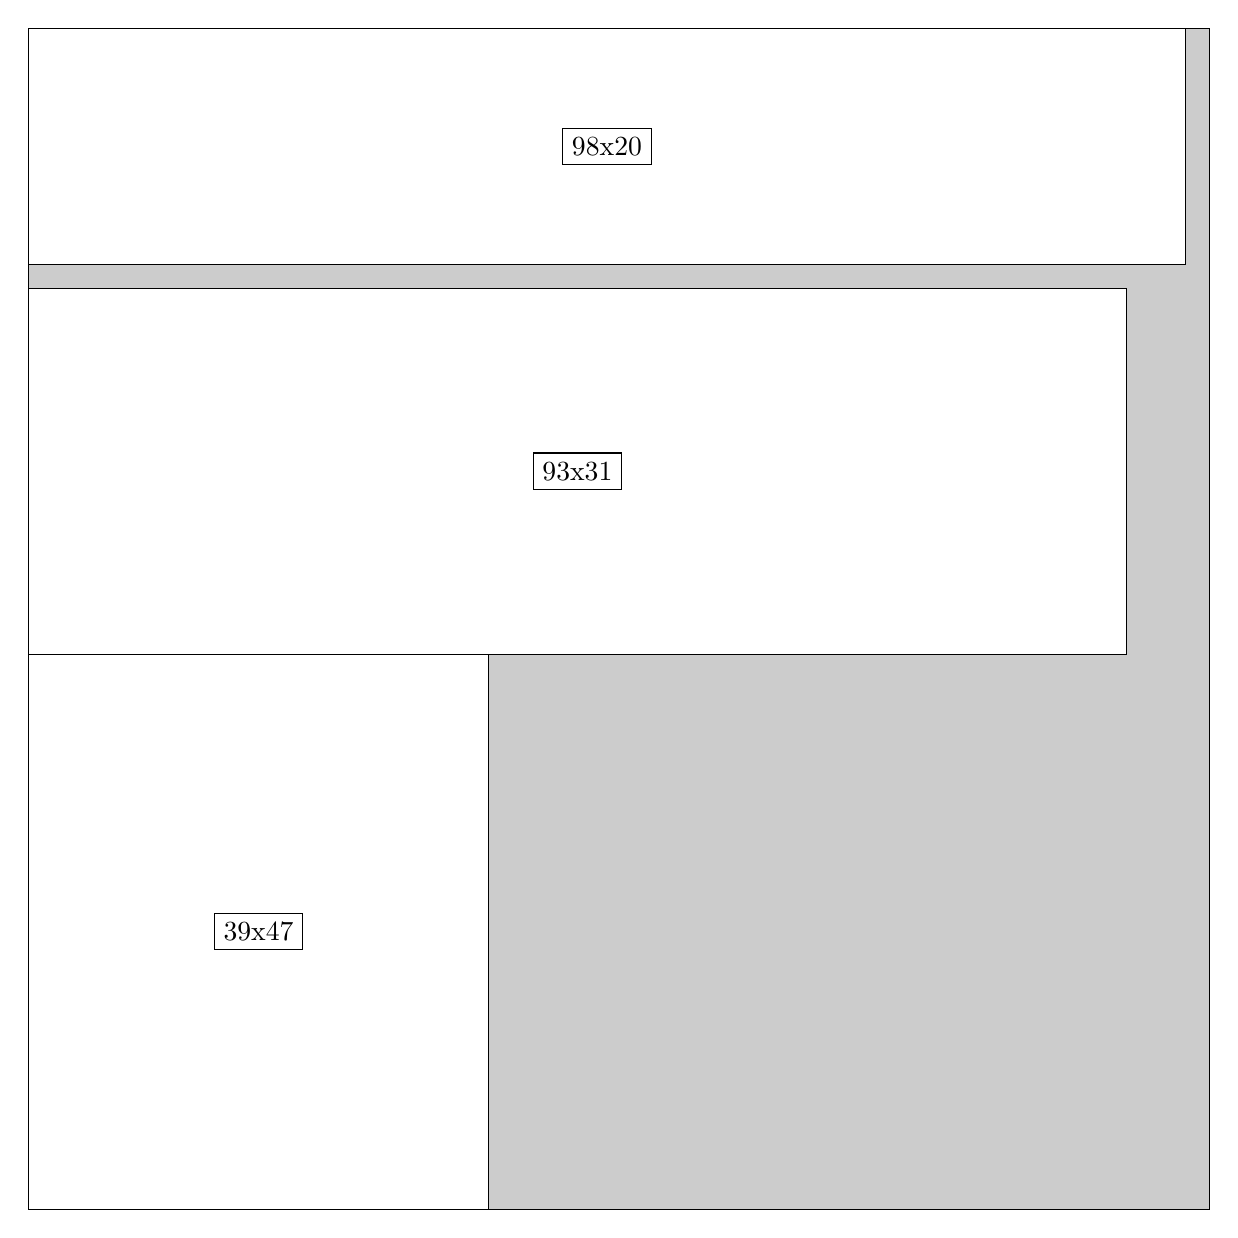
\begin{tikzpicture}[shorten >=1pt,scale=1.0,every node/.style={scale=1.0},->]
\tikzstyle{vertex}=[circle,fill=black!25,minimum size=14pt,inner sep=0pt]
\filldraw[fill=gray!40!white, draw=black] (0,0) rectangle (15.0,15.0);
\foreach \name/\x/\y/\w/\h in {93x31/0.0/7.05/13.95/4.6499999999999995,98x20/0.0/12.0/14.7/3.0,39x47/0.0/0.0/5.85/7.05}
\filldraw[fill=white!40!white, draw=black] (\x,\y) rectangle node[draw] (\name) {\name} ++(\w,\h);
\end{tikzpicture}


w =93 , h =31 , x =0 , y =47 , v =2883
\par
w =98 , h =20 , x =0 , y =80 , v =1960
\par
w =39 , h =47 , x =0 , y =0 , v =1833
\par
\newpage


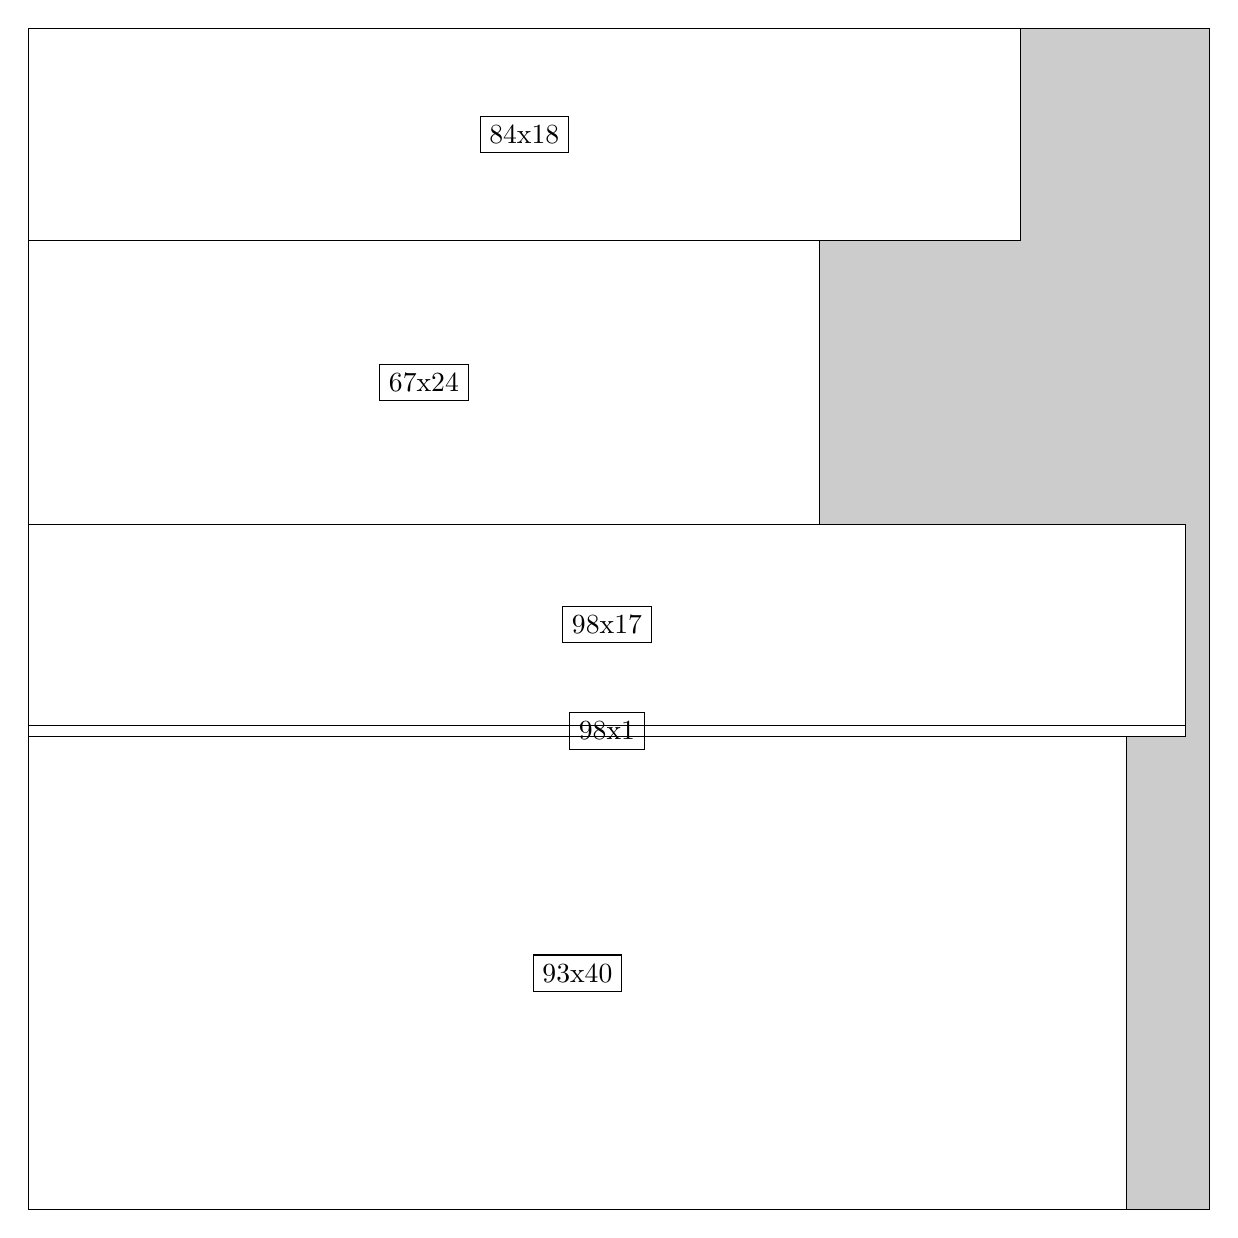
\begin{tikzpicture}[shorten >=1pt,scale=1.0,every node/.style={scale=1.0},->]
\tikzstyle{vertex}=[circle,fill=black!25,minimum size=14pt,inner sep=0pt]
\filldraw[fill=gray!40!white, draw=black] (0,0) rectangle (15.0,15.0);
\foreach \name/\x/\y/\w/\h in {93x40/0.0/0.0/13.95/6.0,67x24/0.0/8.7/10.049999999999999/3.5999999999999996,98x17/0.0/6.1499999999999995/14.7/2.55,84x18/0.0/12.299999999999999/12.6/2.6999999999999997,98x1/0.0/6.0/14.7/0.15}
\filldraw[fill=white!40!white, draw=black] (\x,\y) rectangle node[draw] (\name) {\name} ++(\w,\h);
\end{tikzpicture}


w =93 , h =40 , x =0 , y =0 , v =3720
\par
w =67 , h =24 , x =0 , y =58 , v =1608
\par
w =98 , h =17 , x =0 , y =41 , v =1666
\par
w =84 , h =18 , x =0 , y =82 , v =1512
\par
w =98 , h =1 , x =0 , y =40 , v =98
\par
\newpage


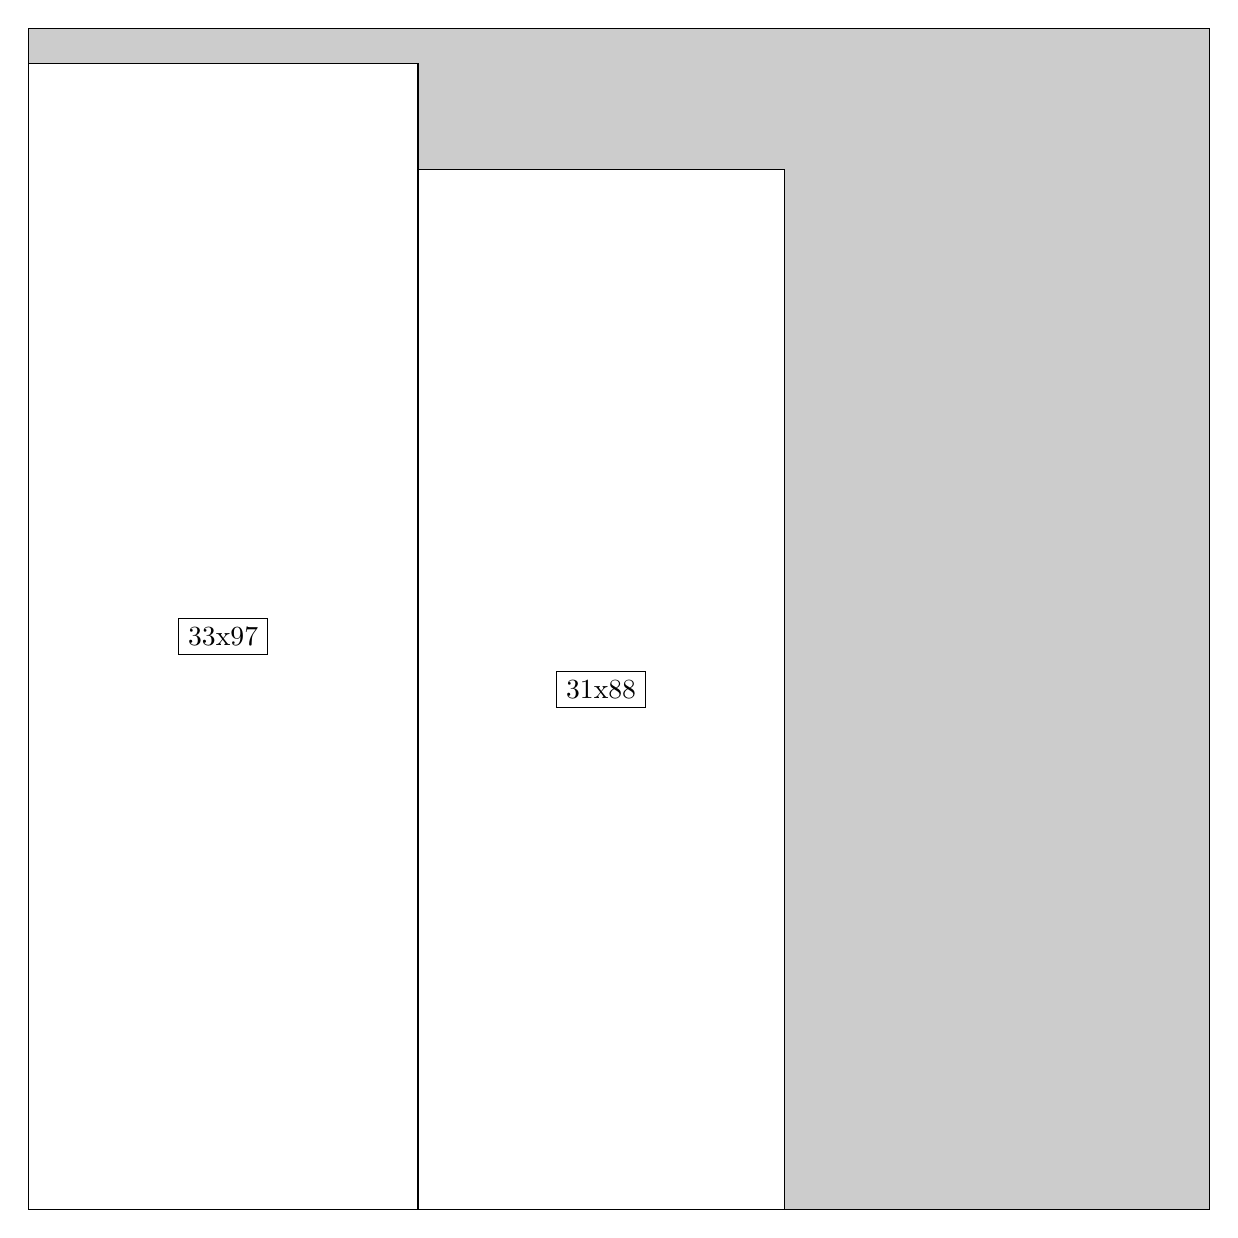
\begin{tikzpicture}[shorten >=1pt,scale=1.0,every node/.style={scale=1.0},->]
\tikzstyle{vertex}=[circle,fill=black!25,minimum size=14pt,inner sep=0pt]
\filldraw[fill=gray!40!white, draw=black] (0,0) rectangle (15.0,15.0);
\foreach \name/\x/\y/\w/\h in {33x97/0.0/0.0/4.95/14.549999999999999,31x88/4.95/0.0/4.6499999999999995/13.2}
\filldraw[fill=white!40!white, draw=black] (\x,\y) rectangle node[draw] (\name) {\name} ++(\w,\h);
\end{tikzpicture}


w =33 , h =97 , x =0 , y =0 , v =3201
\par
w =31 , h =88 , x =33 , y =0 , v =2728
\par
\newpage


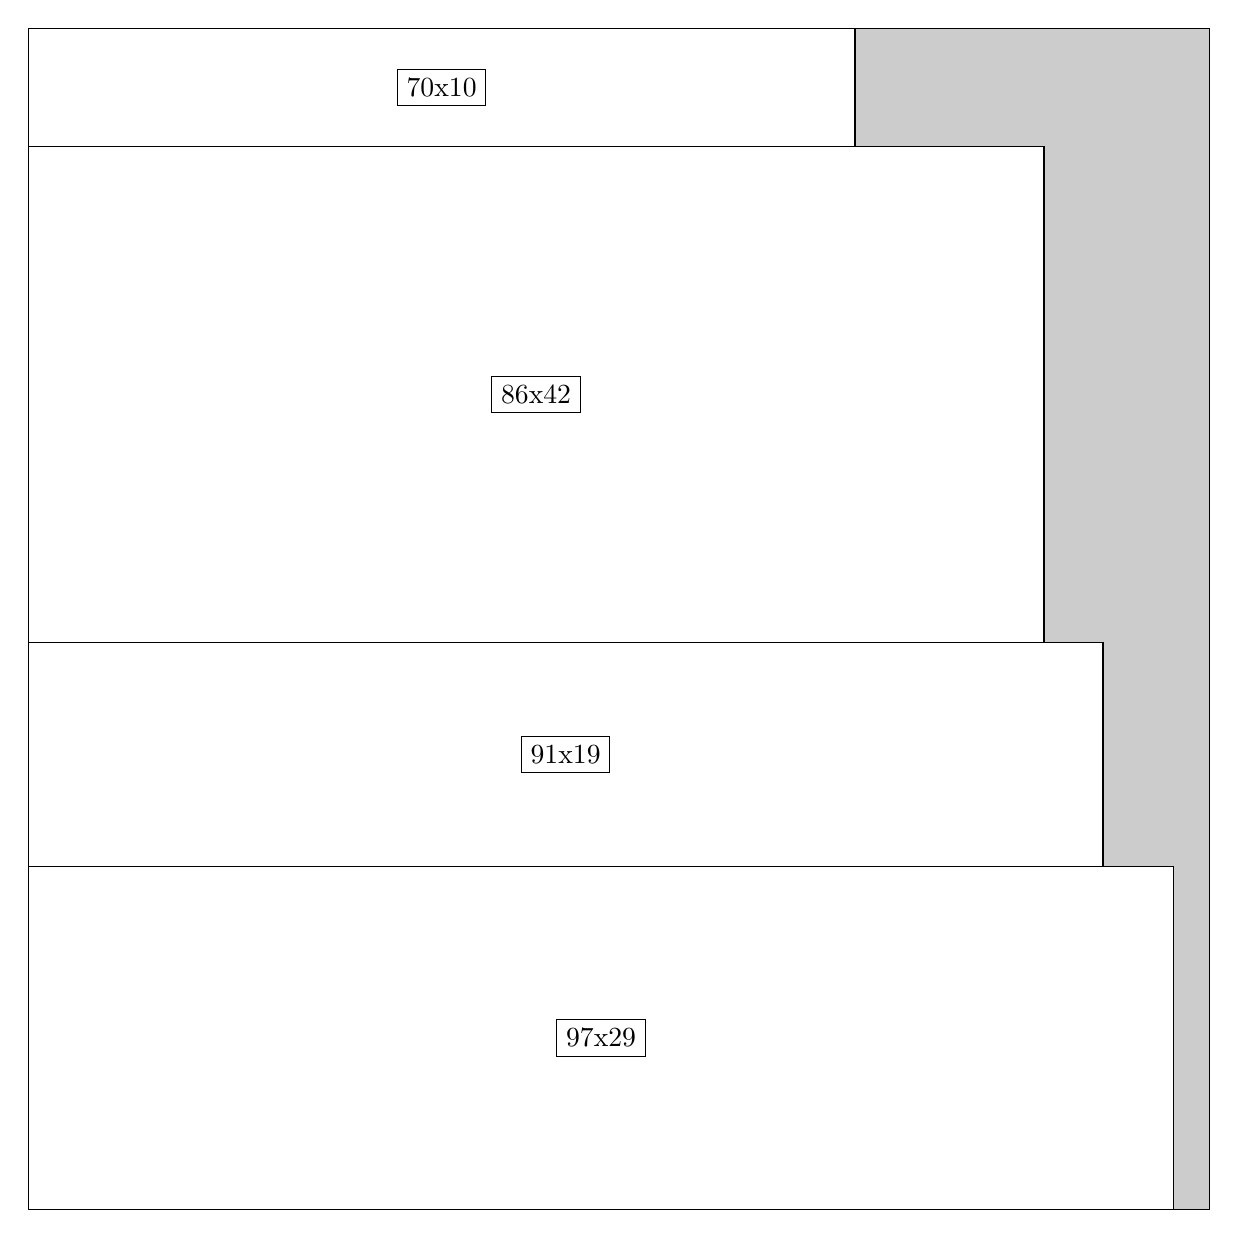
\begin{tikzpicture}[shorten >=1pt,scale=1.0,every node/.style={scale=1.0},->]
\tikzstyle{vertex}=[circle,fill=black!25,minimum size=14pt,inner sep=0pt]
\filldraw[fill=gray!40!white, draw=black] (0,0) rectangle (15.0,15.0);
\foreach \name/\x/\y/\w/\h in {86x42/0.0/7.199999999999999/12.9/6.3,97x29/0.0/0.0/14.549999999999999/4.35,91x19/0.0/4.35/13.65/2.85,70x10/0.0/13.5/10.5/1.5}
\filldraw[fill=white!40!white, draw=black] (\x,\y) rectangle node[draw] (\name) {\name} ++(\w,\h);
\end{tikzpicture}


w =86 , h =42 , x =0 , y =48 , v =3612
\par
w =97 , h =29 , x =0 , y =0 , v =2813
\par
w =91 , h =19 , x =0 , y =29 , v =1729
\par
w =70 , h =10 , x =0 , y =90 , v =700
\par
\newpage


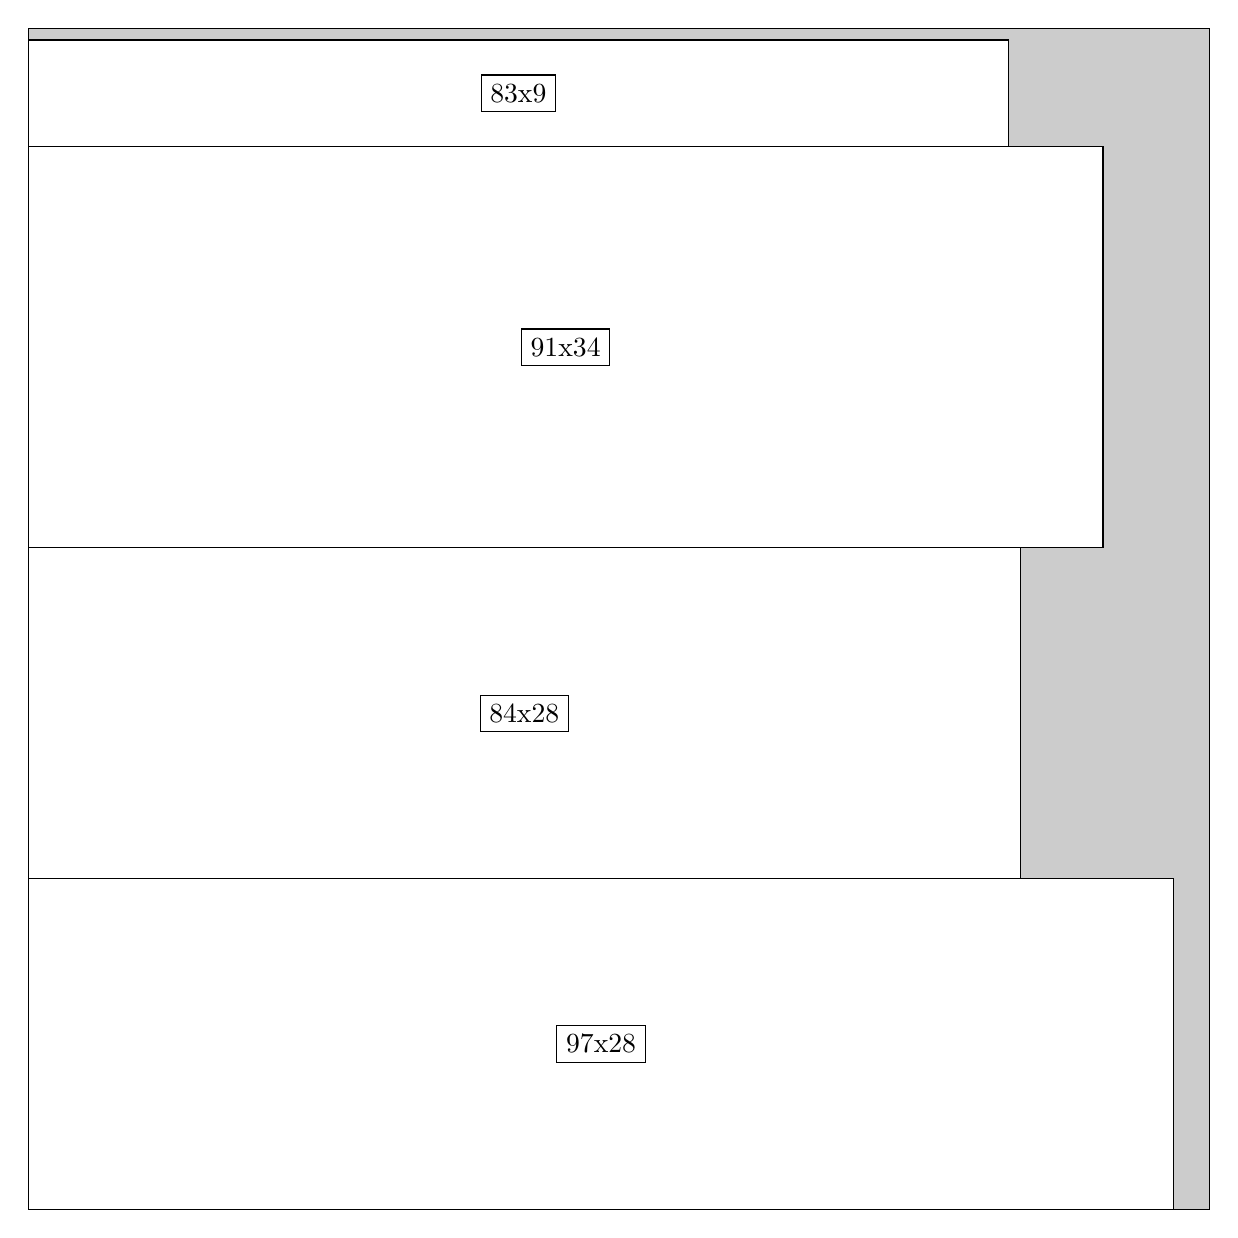
\begin{tikzpicture}[shorten >=1pt,scale=1.0,every node/.style={scale=1.0},->]
\tikzstyle{vertex}=[circle,fill=black!25,minimum size=14pt,inner sep=0pt]
\filldraw[fill=gray!40!white, draw=black] (0,0) rectangle (15.0,15.0);
\foreach \name/\x/\y/\w/\h in {91x34/0.0/8.4/13.65/5.1,84x28/0.0/4.2/12.6/4.2,97x28/0.0/0.0/14.549999999999999/4.2,83x9/0.0/13.5/12.45/1.3499999999999999}
\filldraw[fill=white!40!white, draw=black] (\x,\y) rectangle node[draw] (\name) {\name} ++(\w,\h);
\end{tikzpicture}


w =91 , h =34 , x =0 , y =56 , v =3094
\par
w =84 , h =28 , x =0 , y =28 , v =2352
\par
w =97 , h =28 , x =0 , y =0 , v =2716
\par
w =83 , h =9 , x =0 , y =90 , v =747
\par
\newpage


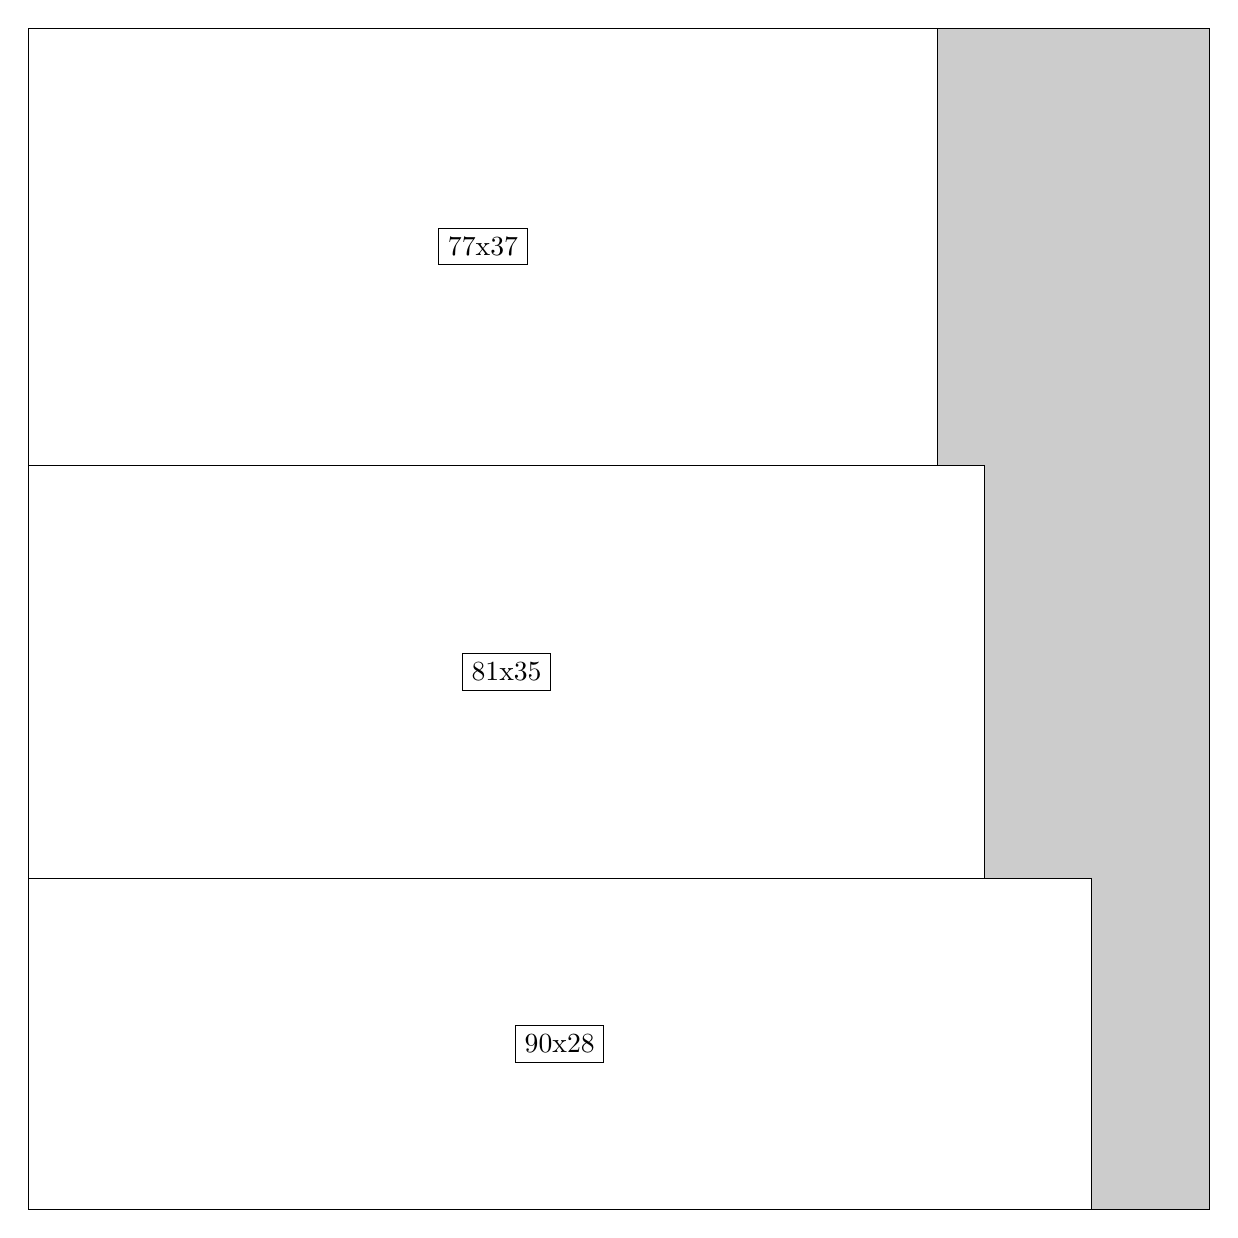
\begin{tikzpicture}[shorten >=1pt,scale=1.0,every node/.style={scale=1.0},->]
\tikzstyle{vertex}=[circle,fill=black!25,minimum size=14pt,inner sep=0pt]
\filldraw[fill=gray!40!white, draw=black] (0,0) rectangle (15.0,15.0);
\foreach \name/\x/\y/\w/\h in {77x37/0.0/9.45/11.549999999999999/5.55,81x35/0.0/4.2/12.15/5.25,90x28/0.0/0.0/13.5/4.2}
\filldraw[fill=white!40!white, draw=black] (\x,\y) rectangle node[draw] (\name) {\name} ++(\w,\h);
\end{tikzpicture}


w =77 , h =37 , x =0 , y =63 , v =2849
\par
w =81 , h =35 , x =0 , y =28 , v =2835
\par
w =90 , h =28 , x =0 , y =0 , v =2520
\par
\newpage


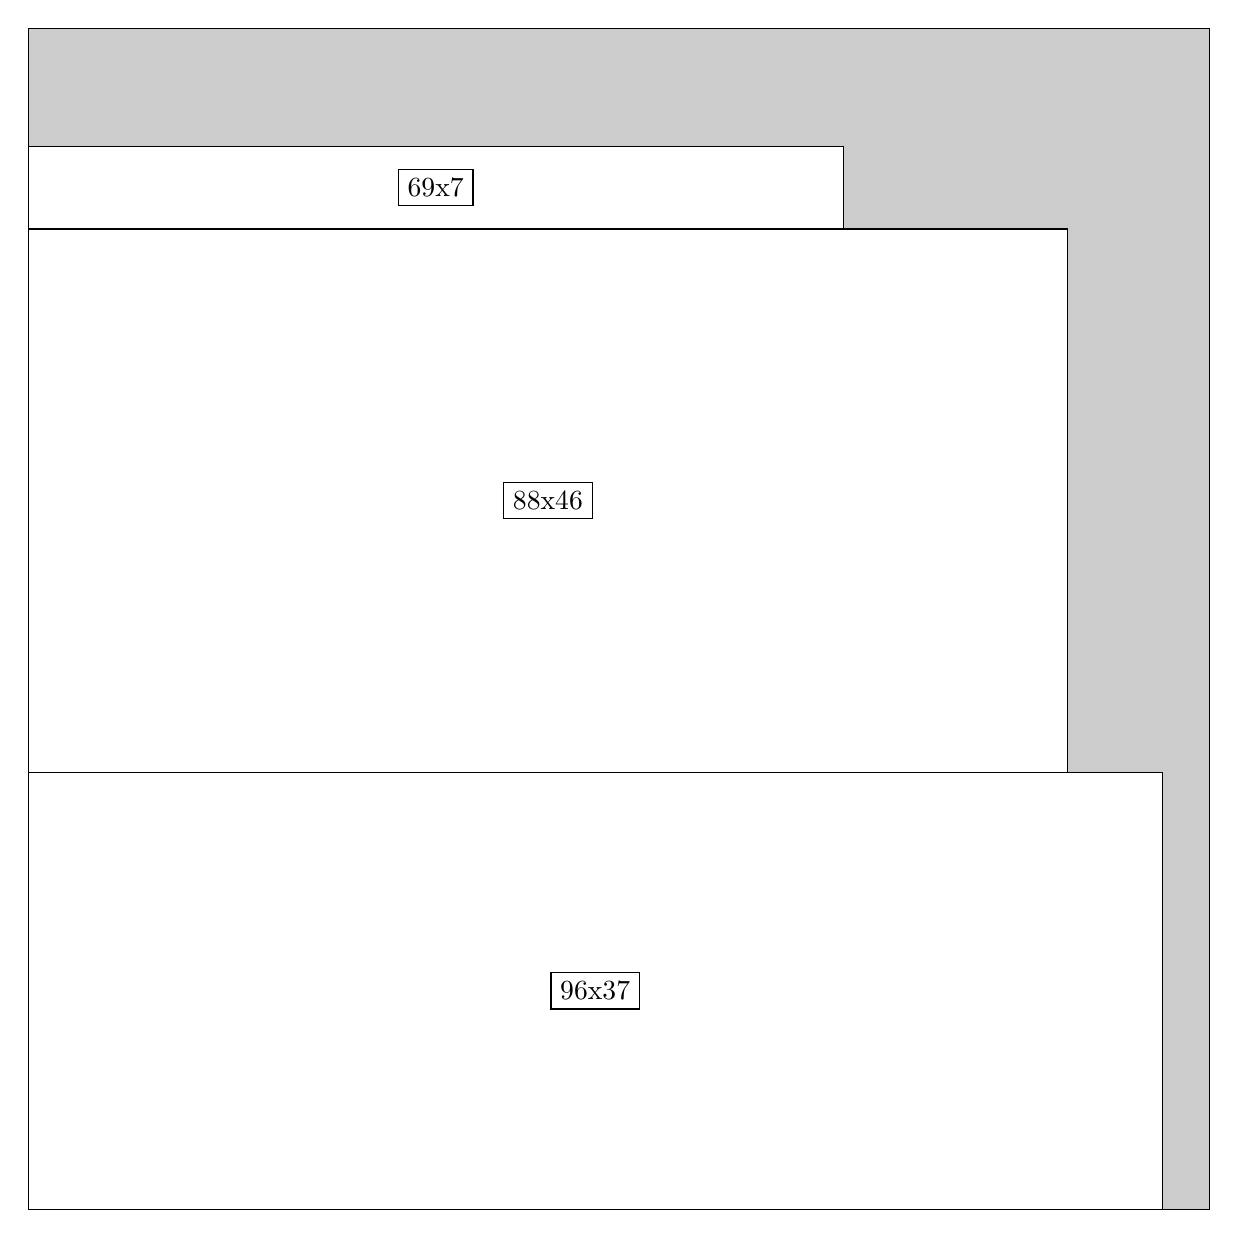
\begin{tikzpicture}[shorten >=1pt,scale=1.0,every node/.style={scale=1.0},->]
\tikzstyle{vertex}=[circle,fill=black!25,minimum size=14pt,inner sep=0pt]
\filldraw[fill=gray!40!white, draw=black] (0,0) rectangle (15.0,15.0);
\foreach \name/\x/\y/\w/\h in {96x37/0.0/0.0/14.399999999999999/5.55,88x46/0.0/5.55/13.2/6.8999999999999995,69x7/0.0/12.45/10.35/1.05}
\filldraw[fill=white!40!white, draw=black] (\x,\y) rectangle node[draw] (\name) {\name} ++(\w,\h);
\end{tikzpicture}


w =96 , h =37 , x =0 , y =0 , v =3552
\par
w =88 , h =46 , x =0 , y =37 , v =4048
\par
w =69 , h =7 , x =0 , y =83 , v =483
\par
\newpage


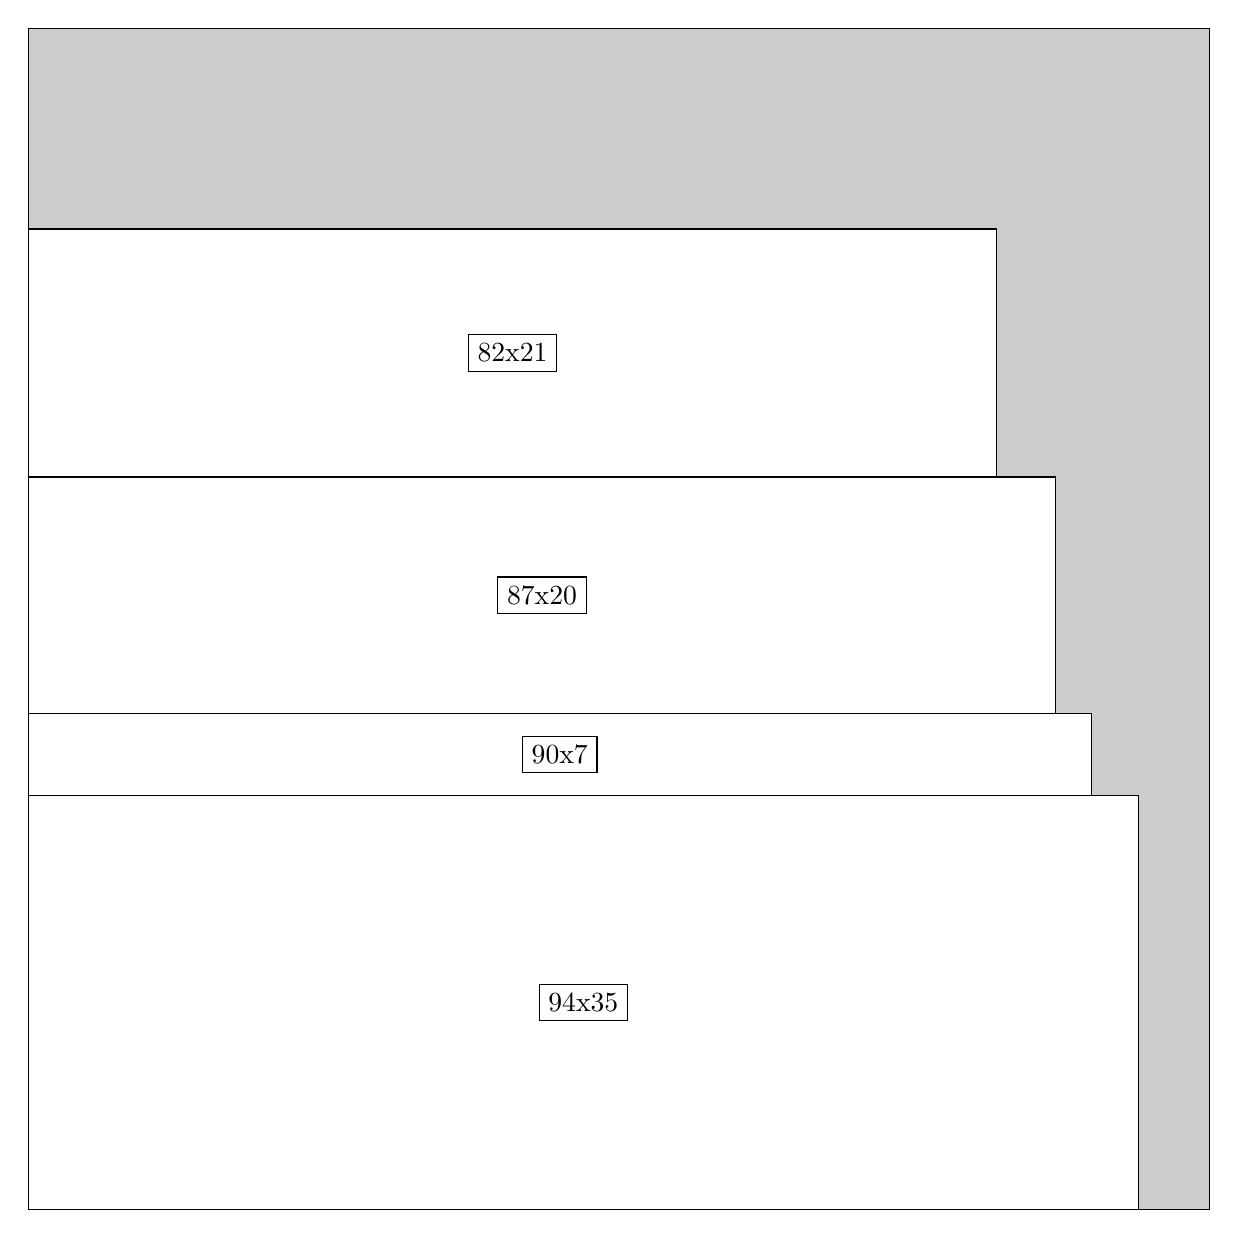
\begin{tikzpicture}[shorten >=1pt,scale=1.0,every node/.style={scale=1.0},->]
\tikzstyle{vertex}=[circle,fill=black!25,minimum size=14pt,inner sep=0pt]
\filldraw[fill=gray!40!white, draw=black] (0,0) rectangle (15.0,15.0);
\foreach \name/\x/\y/\w/\h in {94x35/0.0/0.0/14.1/5.25,87x20/0.0/6.3/13.049999999999999/3.0,82x21/0.0/9.299999999999999/12.299999999999999/3.15,90x7/0.0/5.25/13.5/1.05}
\filldraw[fill=white!40!white, draw=black] (\x,\y) rectangle node[draw] (\name) {\name} ++(\w,\h);
\end{tikzpicture}


w =94 , h =35 , x =0 , y =0 , v =3290
\par
w =87 , h =20 , x =0 , y =42 , v =1740
\par
w =82 , h =21 , x =0 , y =62 , v =1722
\par
w =90 , h =7 , x =0 , y =35 , v =630
\par
\newpage


\end{document}